\section{Modifications to Programmable MBIST}
\label{sect:bg-modifications}
This report proposes to make enhancements to the base design.  The proposed design will introduce programmable CMs in the AG.  It will also show that replacing the auxiliary memory with a data pattern generator can achieve a reduction in area.

\subsection{Address Generator Expansion}
The address generator originally supported linear and pseudo-random address counting methods.  The design in this report will add Gray code, address complement and 2\textsuperscript{\textit{i}} CMs.  The new CMs are generated through logic gates using the linear counter output.  Table \ref{tab:ac} provides an example of the address complement design and Table \ref{tab:gc} shows the same for the Gray code design.  In these tables, \textit{A\textsubscript{3:0}} is the next address and \textit{C\textsubscript{3:0}} is the current output of the linear counter.

\begin{table}[H]
  \centering
  \caption[Address Complement CM Algorithm]{Address Complement Algorithm for 4-bit Address Lines}
  \begin{tabular}{|l|l|}
    \hline
    \multicolumn{2}{|c|}{Address Complement} \\
    \hline  
    Up  & Down  \\                                                          
    \hline
    A\textsubscript{3} = C\textsubscript{0}                           & A\textsubscript{3} = $\overline{C\textsubscript{0}}$              \\ %ac3
    A\textsubscript{2} = C\textsubscript{3} $\oplus$ C\textsubscript{0} & A\textsubscript{2} = C\textsubscript{3} $\oplus$ C\textsubscript{0} \\ %ac2
    A\textsubscript{1} = C\textsubscript{2} $\oplus$ C\textsubscript{0} & A\textsubscript{1} = C\textsubscript{2} $\oplus$ C\textsubscript{0} \\ %ac1
    A\textsubscript{0} = C\textsubscript{1} $\oplus$ C\textsubscript{0} & A\textsubscript{0} = C\textsubscript{1} $\oplus$ C\textsubscript{0} \\ %ac0
    \hline
  \end{tabular} 
  \label{tab:ac}
\end{table}

\begin{table}[H]
  \centering
  \caption[Gray Code CM Algorithm]{Gray Code Algorithm for 4-bit Address Lines}
  \begin{tabular}{|l|l|}
    \hline
    \multicolumn{2}{|c|}{Gray Coding} \\
    \hline  
    Up & Down \\
    \hline
    A\textsubscript{3} = C\textsubscript{3}                           & A\textsubscript{3} = $\overline{C\textsubscript{3}}$              \\ %gc3
    A\textsubscript{2} = C\textsubscript{3} $\oplus$ C\textsubscript{2} & A\textsubscript{2} = C\textsubscript{3} $\oplus$ C\textsubscript{2} \\ %gc2
    A\textsubscript{1} = C\textsubscript{2} $\oplus$ C\textsubscript{1} & A\textsubscript{1} = C\textsubscript{2} $\oplus$ C\textsubscript{1} \\ %gc1
    A\textsubscript{0} = C\textsubscript{1} $\oplus$ C\textsubscript{0} & A\textsubscript{0} = C\textsubscript{1} $\oplus$ C\textsubscript{0} \\ %gc0
    \hline  
  \end{tabular}
  \label{tab:gc}
\end{table} 

In addition to the address complement and Gray code CMs, the 2\textsuperscript{\textit{i}} CM is added to enable the MOVI memory test.  For \textit{N} address lines, the regular 2\textsuperscript{\textit{i}} CM requires a total of \textit{2}x\textit{N}x\textit{N}=\textit{2N}\textsuperscript{i} mux inputs.  This number can be reduced to \textit{2N}+(\textit{2}x\textit{2}x\textit{N})=\textit{6N} mux inputs using the minimal 2\textsuperscript{\textit{i}} CM \cite{5941430}.  Table \ref{tab:2i} provides an example of the regular and minimal solution for a 4-bit address line.  In the regular solution, the address columns are rotating to the left as \textit{i} increases.  This requires a 4-input mux on each of the 4 address lines plus an additional input required for up/down address direction.  The minimal solution recognizes the C\textsubscript{0} input toggels on each count and interchanges the C\textsubscript{\textit{i}} column with the C{\textsubscript{0}} column.  

\begin{table}[H]
  \caption{2\textsuperscript{\textit{i}} Addressing Example}
  \centering
  \begin{tabular}{|c||c|c|c|c||c|c|c|c|}
  \hline
    \multicolumn{1}{|c||}{} & 
    \multicolumn{4}{|c||}{Regular 2\textsuperscript{\textit{i}}} &
    \multicolumn{4}{|c|}{Minimal 2\textsuperscript{\textit{i}}} \\
  \hline
   \textit{num.}&  0 &             1 &             2 &             3 &             0 &             1 &             2 &             3 \\
   \hline
   0 & 000\textbf{0} & 00\textbf{0}0 & 0\textbf{0}00 & \textbf{0}000 & 000\textbf{0} & 00\textbf{0}0 & 0\textbf{0}00 & \textbf{0}000 \\  
   1 & 000\textbf{1} & 00\textbf{1}0 & 0\textbf{1}00 & \textbf{1}000 & 000\textbf{1} & 00\textbf{1}0 & 0\textbf{1}00 & \textbf{1}000 \\  
   2 & 001\textbf{0} & 01\textbf{0}0 & 1\textbf{0}00 & \textbf{0}001 & 001\textbf{0} & 00\textbf{0}1 & 0\textbf{0}10 & \textbf{0}010 \\  
   3 & 001\textbf{1} & 01\textbf{1}0 & 1\textbf{1}00 & \textbf{1}001 & 001\textbf{1} & 00\textbf{1}1 & 0\textbf{1}10 & \textbf{1}010 \\  
   \hline                                                                          
   4 & 010\textbf{0} & 10\textbf{0}0 & 0\textbf{0}01 & \textbf{0}010 & 010\textbf{0} & 01\textbf{0}0 & 0\textbf{0}01 & \textbf{0}100 \\  
   5 & 010\textbf{1} & 10\textbf{1}0 & 0\textbf{1}01 & \textbf{1}010 & 010\textbf{1} & 01\textbf{1}0 & 0\textbf{1}01 & \textbf{1}100 \\  
   6 & 011\textbf{0} & 11\textbf{0}0 & 1\textbf{0}01 & \textbf{0}011 & 011\textbf{0} & 01\textbf{0}1 & 0\textbf{0}11 & \textbf{0}110 \\  
   7 & 011\textbf{1} & 11\textbf{1}0 & 1\textbf{1}01 & \textbf{1}011 & 011\textbf{1} & 01\textbf{1}1 & 0\textbf{1}11 & \textbf{1}110 \\  
   \hline                                                                          
   8 & 100\textbf{0} & 00\textbf{0}1 & 0\textbf{0}10 & \textbf{0}100 & 100\textbf{0} & 10\textbf{0}0 & 1\textbf{0}00 & \textbf{0}001 \\  
   9 & 100\textbf{1} & 00\textbf{1}1 & 0\textbf{1}10 & \textbf{1}100 & 100\textbf{1} & 10\textbf{1}0 & 1\textbf{1}00 & \textbf{1}001 \\  
  10 & 101\textbf{0} & 01\textbf{0}1 & 1\textbf{0}10 & \textbf{0}101 & 101\textbf{0} & 10\textbf{0}1 & 1\textbf{0}10 & \textbf{0}011 \\  
  11 & 101\textbf{1} & 01\textbf{1}1 & 1\textbf{1}10 & \textbf{1}101 & 101\textbf{1} & 10\textbf{1}1 & 1\textbf{1}10 & \textbf{1}011 \\  
  \hline                                                                           
  12 & 110\textbf{0} & 10\textbf{0}1 & 0\textbf{0}11 & \textbf{0}110 & 110\textbf{0} & 11\textbf{0}0 & 1\textbf{0}01 & \textbf{0}101 \\  
  13 & 110\textbf{1} & 10\textbf{1}1 & 0\textbf{1}11 & \textbf{1}110 & 110\textbf{1} & 11\textbf{1}0 & 1\textbf{1}01 & \textbf{1}101 \\  
  14 & 111\textbf{0} & 11\textbf{0}1 & 1\textbf{0}11 & \textbf{0}111 & 111\textbf{0} & 11\textbf{0}1 & 1\textbf{0}11 & \textbf{0}111 \\  
  15 & 111\textbf{1} & 11\textbf{1}1 & 1\textbf{1}11 & \textbf{1}111 & 111\textbf{1} & 11\textbf{1}1 & 1\textbf{1}11 & \textbf{1}111 \\  
  \hline
  \end{tabular}
  \label{tab:2i}
\end{table}

\subsection{Programmable Address Generator}
The original design did not use the address mode field in the IR.  It also did not specify what type of counter to use for the address counter.  The designerhad to decide whether to implement the pseudo-random or linear counter, and use that as the CM for tests.  The only programmability for address was the direction which was set using the up/down field in the IR.  This report adds the ability to select which address generation pattern to use.  The IR was expanded with new fields for AG modes to allow programmability, and the instruction field is decoded within the BIST to select the address counting method.  Table \ref{tab:addrmode} lists the new address mode operation codes.

\begin{table}[H]
  \caption{PMBIST Address Modes}
  \centering
 \begin{tabular}{|p{1in}|p{0.75in}|p{3in}|}
  \hline
  Name & Op Code (binary) & Description \\ [0.5ex]
  \hline\hline
  Linear              & 0000 & Standard numerical sequence  \\ 
  \hline
  Pseudo-Random       & 0001 & Repeatable random sequence \\ 
  \hline
  Address \ Complement  & 0010 & Progresses linearly on even steps and inverts all bits on odd steps.\\ 
  \hline
  \textit{Reserved}            & 01XX & Available for additional addressing modes \\ 
  \hline
  Gray Coding         & 0011 & Changes only one bit per address transition \\ 
  \hline
  2\textsuperscript{\textit{i}}& 1[j\textsubscript{2:0}] & Generates all address pairs with a \textit{Hamming} distance of 1.  2\textsuperscript{\textit{i}} = \textit{j}\textsubscript{2:0} where \textit{i} is the position of the address bit that determines address-pair for \textit{Hamming} distance. \\ 
  \hline
 \end{tabular}
\label{tab:addrmode}
\end{table}

\subsection{Dynamic Background Pattern Generation}
\label{sec:dg}
The auxiliary memory is used to store NPSF background patterns in the base design.  To reduce the area required by this design, the auxiliary memory is replaced by a dynamic background pattern generator.  The generator creates the Type-1 neighborhood pattern and translates it to an 8-bit value that can be written sequentially to memory to create the background pattern.

\begin{figure}[H]
  \centering
  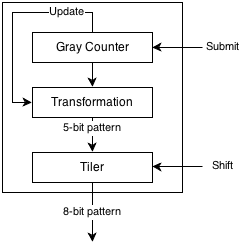
\includegraphics[scale=0.5]{datagen}
  \caption{Data Generator Block Diagram}
  \label{fig:datagen}
\end{figure}
The data generator block design is shown in Figure \ref{fig:datagen}.  The Gray counter is a 5-bit counter that generates gray code and repeats after 32 iterations.  The gray code is passed to the transform block which converts the code to a Eulerian Sequence.  A detailed description of the Euler Sequence can be found in \cite{1675556}.  Essentially, a 5-bit Euler Sequence used as the Type-1 NPSF background will transition through all the possible read and write combinations that could occur.  This requires 161 different sequences which can be broken into five groupings as shown in \ref{tab:euler}.  Except for the first column, each column is generated by a one-bit right shift and rotate followed by inverting the most and least significant bits \cite{957583}.

\begin{table}[H]
  \caption{Partial 5-bit Euler Sequence}
  \centering
  \begin{tabular}{c c c c c c}
  \hline\hline
  Iteration    & Gray (E[0]) & E[1]  & E[2]  & E[3]  & E[4]  \\
  X0  & 00000 & 10001 & 01001 & 00101 & 00011 \\
  X1  & 00001 & 00001 & 00001 & 00001 & 00001 \\
  X2  & 00011 & 00000 & 10001 & 01001 & 00101 \\
  ......             & ...   & ...   & ...   & ...   & ...   \\
  X29 & 10011 & 01000 & 10101 & 01011 & 00100 \\
  X30 & 10001 & 01001 & 00101 & 00011 & 00000 \\
  X31 & 10000 & 11001 & 01101 & 00111 & 00010 \\ [0.5ex]
  \end{tabular}
  \label{tab:euler}
\end{table}

The transformation block provides the 5-bit Euler Sequence to be used as the NPSF background.  To write this value to memory using the Type-1 tiling method, the sequence must be spread over the adjacent rows to create the correct tiling background as shown in \ref{fig:tiling}.  

\begin{figure}[H]
  \centering
  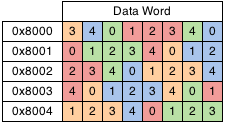
\includegraphics[scale=0.5]{type1tiling}
  \caption[Type-1 Neighborhood Tiling Method for Design]{Type-1 Neighborhood Tiling Method for Design}  
   Each 5-bit color block represents one Type-1 neighborhood.
  \label{fig:tiling}
\end{figure}


